\documentclass[11pt,oneside]{book}

%%%%%%%%%%%%% Geometry
\usepackage[a4paper,left=2.5cm,right=2.5cm, bottom=2.5cm,top=2.5cm]{geometry}

%%%%%%%%%%%%%%% Les paquets

\usepackage[english]{babel}
\usepackage[palette=MATa]{nexus}
\usepackage{amsmath}
\usepackage{amssymb}
\usepackage{amsthm}
\usepackage{amsfonts}
\usepackage{multirow}
\usepackage{float}
\usepackage{diagbox}
\usepackage{xcolor}
\usepackage{caption}
\usepackage{graphicx}
\usepackage{subfigure}
\graphicspath{{img/}}
\usepackage{paralist}
\usepackage{tikz}
\usepackage{tikz-cd}
\usepackage{urtheorem}
%%%%%%%%%%%%%%%% hyperref
\usepackage{lipsum}
\usepackage[verbose]{hyperref}
\hypersetup{ 
    hidelinks
}
\setlength{\XeTeXLinkMargin}{-1pt}


\begin{document}

\pagestyle{empty}

\definecolor{plop}{HTML}{4D7186}
\begin{textblock}{1}(0,0)
    \noindent\textcolor{plop}{\rule{\paperwidth}{.55\paperheight}}
\end{textblock}


\begin{textblock}{1}(0,.55)
    \noindent\textcolor{black}{\rule{\paperwidth}{.45\paperheight}}
\end{textblock}


\begin{textblock}{1}(.1,.09)
    \noindent{\fontsize{24.88}{2}\selectfont
        \bfseries\textcolor{white}{Algebra}}
\end{textblock}

\begin{textblock}{1}(.1,.15)
    \noindent {\fontsize{24.88}{2}\selectfont
    \bfseries\textcolor{white}{Definitions and Theorems}}
\end{textblock}


\begin{textblock}{1}(.1,.45)
    \noindent {\fontsize{20.74}{2}\selectfont
        \bfseries\textcolor{white}{Assjock}}
\end{textblock}



\begin{textblock}{.9}(.05,.56)
    \begin{flushright}
        \noindent {\fontsize{20.74}{2}\selectfont
            \bfseries\textcolor{orange}{version 1.1+$\varepsilon$}}
    \end{flushright}
\end{textblock}


\begin{textblock}{.45}(.5,.82)
    \begin{center}
        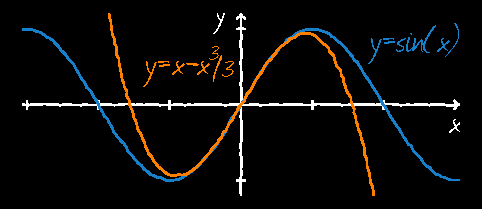
\includegraphics[width=.45\paperwidth]{dlsin}
    \end{center}
\end{textblock}

\begin{textblock}{.4}(.05,.65)
    \begin{center}
        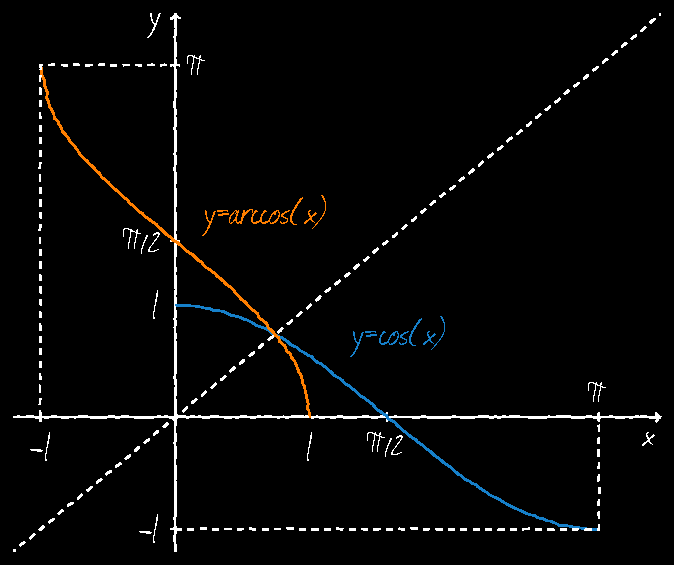
\includegraphics[width=.4\paperwidth]{arccos}
    \end{center}
\end{textblock}


\begin{textblock}{.6}(.05,.6)
    \noindent {\fontsize{20.74}{18}%
    \textcolor{white}{$\displaystyle(a+b)^n = \sum_{k=0}^n 
                \binom{n}{k} a^kb^{n-k}$}}
\end{textblock}


\begin{textblock}{.4}(.4,.77)
    \noindent {\fontsize{17.28}{18}%
    \textcolor{white!80}{$\displaystyle 
                \neg (p\vee q) \equiv (\neg p)\wedge (\neg q)$}}
\end{textblock}

\begin{textblock}{.4}(.1,.93)
    \noindent {\fontsize{14.4}{18}%
    \textcolor{white!50}{$\displaystyle 
                \binom{n}{k} = \frac{n!}{k!(n-k)!}$}}
\end{textblock}


\begin{textblock}{.6}(.5,.69)
    \noindent {\fontsize{17.28}{18}%
    \textcolor{white!10}{$\displaystyle 
                \zeta_k = |a|^{1/n} \mathrm{e}^{i(\mathrm{arg}(a)+2k\pi)/n}$}}
\end{textblock}


\begin{textblock}{.3}(.75,.73)
    \noindent {\fontsize{17.28}{18}%
    \textcolor{white!10}{$\displaystyle \mathrm{e}^{i\pi}+1=0$}}
\end{textblock}



\null\newpage\pagestyle{nexus}

%\tableofcontents
\chapter{Groups}
\section{Logical Symbols}
The logical symbols are a kind of symbols using for theoretical statements.
    \begin{table}[H]
        \centering
        \caption{Frequently-used Logical Symbols}
        \begin{tabular}{|c|c|}\hline
            Symbols&Meanings\\\hline
            $L\Longrightarrow P$& Proposition $L$ is contained in proposition $P$\\
            $L \Longleftrightarrow P $&Proposition $L$ is equivalent to proposition $P$\\
            $\lnot P$&Not $P$\\
            $L\wedge P$&Proposition $L$ and proposition $P$\\
            $L \vee P$&Proposition $L$ or proposition $P$\\
            \hline
        \end{tabular}
    \end{table}
e.g.\[((A\Longrightarrow B)\wedge(\lnot B)\Longrightarrow (\lnot A) )\]


stands for `` if $A$ is contained in  $B$,and $B$ is not true,then $A$ is not true''.

We also call $ A \Longleftrightarrow B$ ``$A$ is the necessary and suffiecent condition of $B$''.

The typical math proposition is like ``$A\Longrightarrow B$''.In order to prove this proposition ,we can use the  implication relationship \[A\Longrightarrow C_1\Longrightarrow \cdots \Longrightarrow C_n\Longrightarrow B\]The every implication relationship in this chain is general truth or proved proposition.

\begin{table}[H]
    \centering
    \caption{Truth Table}
    \begin{tabular}{|c|c|c|c|}
        \hline
        \multirow{2}{*}{$\lnot A$}                       & $A$                    & 0         & 1             \\ \cline{2-4} 
                                                 & $\lnot A$            & 1            & 0             \\ \hline
        \multirow{3}{*}{$A \vee B$}                       &       \diagbox{$A$}{$B$}     &    0        &       1        \\ \cline{2-4} 
                                                 &          0       &   0         &        1        \\ \cline{2-4} 
                                                 &       1         &  1        &        1       \\ \hline
        \multirow{3}{*}{$A \wedge B$}                       &        \diagbox{$A$}{$B$}    &           0&        1          \\ \cline{2-4} 
                                                 &     0         &     0          &      0          \\ \cline{2-4} 
                                                 &        1        &                0       &    1       \\ \hline
        \multirow{3}{*}{$A\Longrightarrow B$}                      &  \diagbox{$A$}{$B$} & 0  &  1 \\ \cline{2-4} 
                                                & 0  &  1 &  1 \\ \cline{2-4} 
                                                & 1  &  0 & 1  \\ \hline
        \end{tabular}
    \end{table}
\begin{question}$\lnot (A\wedge B )\Leftrightarrow (\lnot A \vee \lnot B)$.
\end{question}
\begin{proof}
    (Use the truth table)

    If $A$ is ture, $B$ is ture, $A\wedge B$ is ture. $\lnot (A\wedge B)$ is false.$\lnot A $ is false,$\lnot B$ is false, $(\lnot A \vee \lnot B)$ is false.

    If $A$ is ture, $B$ is false, $A\wedge B$ is false. $\lnot (A\wedge B)$ is true.$\lnot A $ is false,$\lnot B$ is true, $(\lnot A \vee \lnot B)$ is ture.

    If $A$ is flase, $B$ is true, $A\wedge B$ is false. $\lnot (A\wedge B)$ is true.$\lnot A $ is true,$\lnot B$ is false, $(\lnot A \vee \lnot B)$ is ture.

    If $A$ is false, $B$ is false, $A\wedge B$ is false. $\lnot (A\wedge B)$ is true.$\lnot A $ is true,$\lnot B$ is true, $(\lnot A \vee \lnot B)$ is ture.

    So
    \[\lnot (A\wedge B )\Leftrightarrow (\lnot A \vee \lnot B)\]
\end{proof}    

\begin{question}
    $(A \Rightarrow B)\Leftrightarrow\lnot A \vee B$.
\end{question}
\begin{proof}
    Firstly, we confirm the truth of \[(A \Rightarrow B)\Rightarrow\lnot A \vee B\]

    If $(A \Rightarrow B)$ is false, then $\lnot A \vee B$ is true.

    If $(A \Rightarrow B)$ is ture ,then we have two posibilities. The first is $A$ is ture, $B$ is true, so $\lnot A \vee B$ is true. The second is $A$ is false,then $B$ can be true or false, but $\lnot A \vee B$ will be true.

    Hence, $(A \Rightarrow B)\Rightarrow\lnot A \vee B$.

    Secondly, we prove \[(A \Rightarrow B)\Leftarrow\lnot A \vee B\]

    If $\lnot A \vee B$ is false, then $(A \Rightarrow B)$ is true.

    If $\lnot A \vee B$ is true, we have
    \begin{enumerate}
        \item $\lnot A$ is true, $B$ is false, then, $A$ is false, $(A \Rightarrow B)$ is true.
        \item $\lnot A$ is false, $B$ is true, then, $A$ is true, $(A \Rightarrow B)$ is true.
        \item $\lnot A$ is true, $B$ is true, then, $A$ is false, $(A \Rightarrow B)$ is true.
    \end{enumerate}

    So $(A \Rightarrow B)\Leftarrow\lnot A \vee B$.
\end{proof}


\section{Homomorphisms and subgroups}
\begin{ex}
    If $f: G \to H$ is a homomorphism of groups, then $f(e_G) = e_H$ and $f(a^{-1}) = f(a)^{-1}$ for all $a \in G$. Show by example that the first conclusion may be false if $G$, $H$ are monoids that are not groups.
\end{ex}

$$ $$

\begin{ex}
    A group $G$ is abelian if and only if the map $G\to G$ given by $x\to x^{-1}$ is automorphism.
\end{ex}

$$ $$

\begin{ex}
    Let $Q_8$ be the group(under ordinary matrix multiplication) generated by complex matrices $A = \begin{pmatrix}
        0 & 1 \\
        -1 & 0
    \end{pmatrix}$ and $B = \begin{pmatrix}
        0 & i\\
        i & 0
    \end{pmatrix}$, where $i^{2}=-1$. Show that $Q_8$ is a nonabelian group of order 8. $Q_8$ is called the quaternion group.
\end{ex}

$$ $$

\begin{ex}
    Let $H$ be the group(under ordinary matrix multiplication) of real matrices generated by $C = \begin{pmatrix}
        0 & 1\\
        -1 & 0
    \end{pmatrix}$ and $D = \begin{pmatrix}
        0 & 1\\
        1 & 0
    \end{pmatrix}$. Show that $H$ is a nonabelian group of order 8 which is not isomorphic to the quaternion group, but is isomorphic to the group $D_4^*$.
\end{ex}

$$ $$

\begin{ex}
    Let $S$ be a nonempty subset of a group $G$ and define a relation on $G$ by $a ~ b$ if and only if $ab^{-1}\in S$. Show that $~$ is an equivalence relation if and only if $S$ is a subgroup of $G$.
\end{ex}

$$ $$

\begin{ex}
    A nonempty finte subset of a group is s subgroup if and only if it is closed under the product in $G$.
\end{ex}

$$ $$

\begin{ex}
    If $n$ is a fixed integer, then $\{kn | n\in \mathbf{Z}\}\subset\mathbf{Z}$ is an additive subgroup of $\mathbf{Z}$, which is isomorphic to $\mathbf{Z}$. 
\end{ex}

$$ $$

\begin{ex}
    The set $\{\sigma\in S_n | \sigma(n) = n\}$ is a subgroup of $S_n$ which is isomorphic to $S_{n-1}$.
\end{ex}

$$ $$

\begin{ex}
    Let $f: G\to H$ be a homomorphism of groups, $A$ a subgroup of $G$, and $B$ a subgroup of $H$.
    \begin{enumerate}
        \item $\mathrm{Ker} f$ and $f^{-1}(B)$ are subgroups of $G$.
        \item $f(A)$ is a subgroup of $H$.
    \end{enumerate}
\end{ex}

$$ $$

\begin{ex}
    List all subgroups of $Z_2\oplus Z_2$. Is $Z_2\oplus Z_2$ isomorphic to $Z_4$?
\end{ex}

$$ $$

\begin{ex}
    If $G$ is a subgroup, then $C = \{a\in G| ax = xa \text{ for all } x\in G\}$ is a abelian subgroup of $G$. $C$ is called the center of $G$.
\end{ex}

$$ $$

\begin{ex}
    The group $D_4^*$ is not cyclic, but can be generated by two elements. The same is true of $S_n$(nontrivial). What is the minimal number of generators of the additive group $\mathbf{Z}\oplus\mathbf{Z}$?
\end{ex}

$$ $$

\begin{ex}
    If $G = \left\langle a \right\rangle $ is a cyclic group and $H$ is any group, then every homomorphism $f:G\to H$ is completely determined by the element $f(a)\in H$.
\end{ex}

$$ $$

\begin{ex}
    The following cyclic subgroups are all isomorphic: the multiplication group $\left\langle i \right\rangle$ in $\mathbf{C}$, the additive group $\mathbf{Z_4}$ and the subgroup $\left\langle \begin{pmatrix}
        1 & 2 & 3 & 4\\
        2 & 3 & 4 & 1
    \end{pmatrix}\right\rangle$ of $S_4$.
\end{ex}

$$ $$

\begin{ex}
    Let $G$ be a group and $\mathrm{Aut} G$ is the set of all automorphisms of $G$.
    \begin{enumerate}
        \item $\mathrm{Aut} G$ is a group with composition of functions as binary operation.
        \item $\mathrm{Aut} \mathbf{Z}\cong Z_2$ and $\mathrm{Aut} Z_6 \cong Z_2$; $\mathrm{Aut} Z_8\cong Z_2\oplus Z_2$; $\mathrm{Aut} Z_p\cong Z_{p-1}$ ($p$ prime).
        \item What is $\mathrm{Aut Z_n}$ for arbitrary $n\in \mathbf{N^*}$?
    \end{enumerate}
\end{ex}

$$ $$

\begin{ex}
    For each prime $p$ the additive subgroup $Z(p^\infty)$ of $\mathbf{Q}/\mathbf{Z}$ is generated by the set $\{\bar{1/p^n}|n\in \mathbf{N^*}\}$.
\end{ex}

$$ $$

\begin{ex}
    Let $G$ be an abelian group and let $H, K$ be subgroups of $G$. Show that the join $H\vee K$ is the set $\{ab|a\in H, b\in K\}$. Extend this result to any finite number of subgroups of $G$.
\end{ex}

$$ $$

\begin{ex}
    \begin{enumerate}
        \item Let $G$ be a group and $\{H_i| i\in I\}$ a family of subgroups. State and prove a condition that will imply that $\bigcup\limits_{i\in I}H_i$ is a subgroup, that is $\bigcup\limits_{i\in I}H_i = \left\langle\bigcup\limits_{i\in I}H_i\right\rangle$.
        \item Given an example of a group $G$ and a family of subgroups $\{H_i|i \in I\}$ such that $\bigcup\limits_{i\in I}H_i \neq \left\langle\bigcup\limits_{i\in I}H_i\right\rangle$.
    \end{enumerate}
\end{ex}

$$ $$

\begin{ex}
    \begin{enumerate}
        \item The set of all subgroups of a group $G$, partially ordered by set theoretic inclusion, forms a complete lattice in which the g.l.b of $\{H_i|i\in I\}$ is $\bigcap\limits_{i\in I}H_i$ and the l.u.b is $\left\langle\bigcap\limits_{i\in I}H_i\right\rangle$.
        \item Exhibit the lattice of subgroups of the groups $S_3, D_4^*, Z_6, Z_{27}$ and $Z_{36}$.
    \end{enumerate}
\end{ex}
\end{document}